\chapter{Legacy PEO Evaluation System and Results (Pre-2026)}\label{app:legacy_peo_evaluation}

This appendix describes the evaluation mechanism and attainment results of the legacy Program Educational Objective (PEO) evaluation system, referenced in Criterion~1. The full survey forms are reproduced in Appendix~\ref{app:survey_forms}.

\section{Legacy Evaluation Mechanism}

\textcolor{red}{Under the legacy system, each PEO was assessed through a set of Key Performance Indicators (KPIs) derived from annual Alumni and Employer surveys. Indicator design accounted for diversity in graduate career paths e.g., employment, entrepreneurship, or higher education, so that a graduate's choice of path did not itself count against attainment. Each KPI was expressed as the percentage of respondents responding favourably to a specific survey item, with an attainment threshold of 50\% or 60\% depending on the indicator. A PEO was considered attained only if all of its constituent sub-KPIs individually met their respective thresholds, with cumulative PEO attainment computed as the equal-weight average of its sub-KPIs.} Following KPIs were defined in the old scheme.


\noindent\textbf{PEO 1 --- Demonstrate sound software engineering knowledge and skill set.}
\begin{itemize}[leftmargin=1.5em,topsep=2pt]
\item 60\% of respondent employers are satisfied with technical knowledge of employed graduates.
\item 60\% of respondent employers are satisfied with competence and skills of employed graduates.
\item 60\% of respondent graduates gave positive feedback on their knowledge compared to their peers.
\item 60\% of respondent graduates gave positive feedback on their competence compared to their peers.
\item 50\% of respondent graduates are employed within one year of their graduation.
\item 50\% of respondent graduates are pursuing higher education.
\end{itemize}

\noindent\textbf{PEO 2 --- Lead diverse teams and work collaboratively to develop innovative solutions.}
\begin{itemize}[leftmargin=1.5em,topsep=2pt]
\item 60\% of respondent employers are satisfied with the communications skills of employed graduates.
\item 60\% of respondent employers are satisfied with the teamwork skills of employed graduates.
\item 60\% of respondent employers are satisfied with the independent project handling skills of employed graduates.
\item 60\% of respondent graduates are involved in research and/or innovation activities.
\item 60\% of respondent graduates have handled projects independently.
\item 50\% of respondent graduates are involved in professional development activities.
\end{itemize}

\noindent\textbf{PEO 3 --- Conduct professional practice for sustainable development with due consideration for societal, ethical, and environmental aspects.}
\begin{itemize}[leftmargin=1.5em,topsep=2pt]
\item 60\% of respondent employers are satisfied with adherence to ethical values by employed graduates.
\item 60\% of respondent employers are satisfied with the discharge of professional obligations of employed graduates.
\item 50\% of respondent graduates have incorporated UN SDGs in their projects / services / solutions / products etc.
\item 50\% of respondent graduates are involved in projects addressing societal and/or environmental issues.
\end{itemize}

\section{Legacy Evaluation Results (2025)}

Table~\ref{tab:legacy_results} presents the attainment results obtained under the legacy evaluation system, using Alumni and Employer survey data collected in 2025.

\begingroup
\scriptsize
\setlength{\tabcolsep}{4pt}
\renewcommand{\arraystretch}{1.2}
\begin{longtable}[]{@{}>{\raggedright\arraybackslash}p{0.06\textwidth}>{\raggedright\arraybackslash}p{0.52\textwidth}>{\raggedright\arraybackslash}p{0.20\textwidth}>{\centering\arraybackslash}p{0.10\textwidth}@{}}
\caption{Attainment of PEOs under the Legacy Evaluation System (Alumni/Employer surveys, data collected in 2025)}\label{tab:legacy_results}\\
\toprule
\multicolumn{4}{@{}>{\raggedright\arraybackslash}p{0.92\textwidth}@{}}{\textbf{PEO 1}: Demonstrate sound software engineering knowledge and skill set.}\\
\midrule
\textbf{S. No.} & \textbf{KPI} & \textbf{Measurement Tool} & \textbf{Attainment \%}\\
\midrule
\endfirsthead
\toprule
\textbf{S. No.} & \textbf{KPI} & \textbf{Measurement Tool} & \textbf{Attainment \%}\\
\midrule
\endhead
1 & 60\% of respondent employers are satisfied with technical knowledge of employed graduates & Employer Survey (Q1) & 85\%\\
2 & 60\% of respondent employers are satisfied with competence and skills of employed graduates & Employer Survey (Q2) & 86\%\\
3 & 60\% of respondent graduates gave positive feedback on their knowledge compared to their peers & Alumni Survey (Q1) & 76\%\\
4 & 60\% of respondent graduates gave positive feedback on their competence compared to their peers & Alumni Survey (Q2) & 76\%\\
5 & 50\% of respondent graduates are employed within one year of their graduation & Alumni Survey (Q6) & 89\%\\
6 & 50\% of respondent graduates are pursuing higher education & Alumni Survey (Q7) & 36\%\\
\addlinespace
\midrule
\multicolumn{4}{@{}>{\raggedright\arraybackslash}p{0.92\textwidth}@{}}{\textbf{PEO 2}: Lead diverse teams and work collaboratively to develop innovative solutions.}\\
\midrule
\textbf{S. No.} & \textbf{KPI} & \textbf{Measurement Tool} & \textbf{Attainment \%}\\
\midrule
1 & 60\% of respondent employers are satisfied with the communications skills of employed graduates & Employer Survey (Q3) & 84\%\\
2 & 60\% of respondent employers are satisfied with the teamwork skills of employed graduates. & Employer Survey (Q4) & 85\%\\
3 & 60\% of respondent employers are satisfied with the independent project handling skills of employed graduates & Employer Survey (Q5) & 81\%\\
4 & 60\% of respondent graduates are involved in research and/or innovation activities & Alumni Survey (Q3) & 69\%\\
5 & 60\% of respondent graduates have handled projects independently & Alumni Survey (Q4) & 79\%\\
6 & 50\% of respondent graduates are involved in professional development activities & Alumni Survey (Q5) & 76\%\\
\addlinespace
\midrule
\multicolumn{4}{@{}>{\raggedright\arraybackslash}p{0.92\textwidth}@{}}{\textbf{PEO 3}: Conduct professional practice for sustainable development with due consideration for societal, ethical, and environmental aspects.}\\
\midrule
\textbf{S. No.} & \textbf{KPI} & \textbf{Measurement Tool} & \textbf{Attainment \%}\\
\midrule
1 & 60\% of respondent employers are satisfied with adherence to ethical values by employed graduates. & Employer Survey (Q6) & 86\%\\
2 & 60\% of respondent employers are satisfied with the discharge of professional obligations of employed graduates. & Employer Survey (Q7) & 78\%\\
3 & 50\% of respondent graduates have incorporated UN SDGs in their projects / services / solutions / products etc. & Alumni Survey (Q8) & 52\%\\
4 & 50\% of respondent graduates are involved in projects addressing societal and/or environmental issues. & Alumni Survey (Q9) & 64\%\\
\bottomrule
\end{longtable}
\endgroup

Under the legacy criterion requiring every sub-KPI to meet its threshold individually, PEO~2 and PEO~3 were fully attained. For PEO~1, five of the six sub-KPIs exceeded their thresholds. The indicator measuring the proportion of graduates pursuing higher education reached 36\% against a 50\% threshold. On an equal-weight cumulative basis, the attainment levels were approximately 75\%, 79\%, and 70\% for PEO~1, PEO~2, and PEO~3, respectively.

Figure~\ref{fig:legacy_analysis} shows the per-KPI attainment for each PEO under the legacy evaluation system, with the dashed line in each panel indicating the applicable attainment threshold (50\% or 60\%, depending on the indicator). All indicators meet their respective thresholds except PEO~1 KPI-6 (pursuing higher education), which falls below its 50\% threshold.

\begin{figure}[tb]
\centering
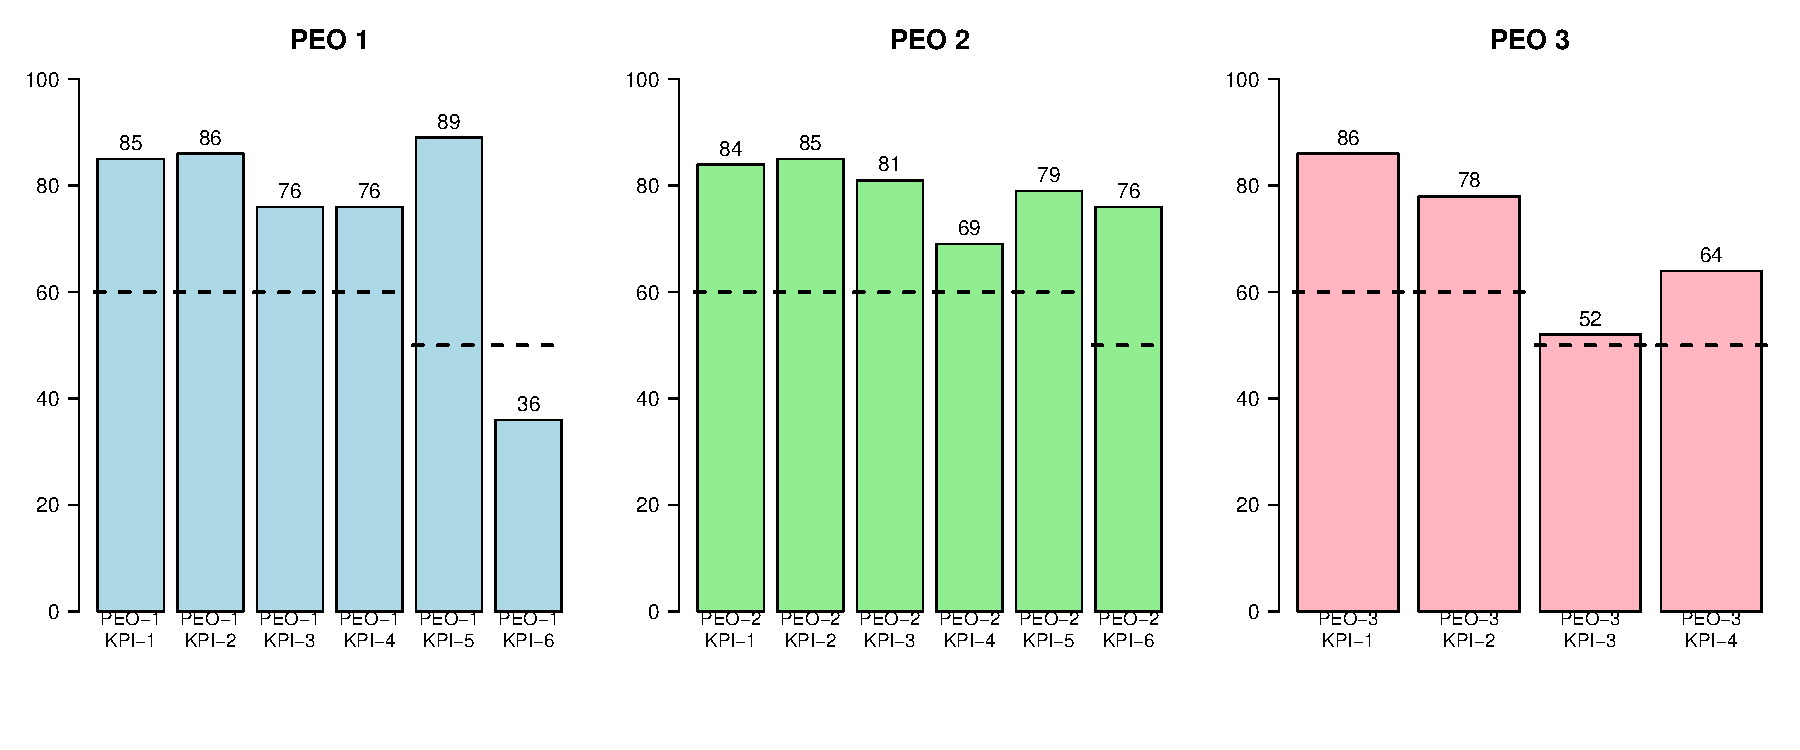
\includegraphics[width=\textwidth]{images/criterion_1/media/legacy_analysis.pdf}
\caption{Per-KPI attainment under the Legacy Evaluation System (data collected in 2025). The dashed line in each panel marks the applicable attainment threshold for that indicator.}
\label{fig:legacy_analysis}
\end{figure}

The single below-threshold indicator reflects a structural limitation of the legacy instrument rather than a shortfall in program outcomes. Pursuit of higher education is a binary indicator that does not, on its own, represent PEO attainment, since graduates who enter employment instead of higher education are not demonstrating a deficiency against the objective. Limitations of this nature where indicators are only loosely aligned with PEO-level outcomes, together with a rigid all-or-nothing pass rule, motivated the revised evaluation system described in Criterion~1.
